
El momento de un mu\'on low-$p_{T}$ es extraido a partir de la reconstrucci\'on de su trayectoria a trav\'es de las señales o hits que deja en el tracker junto con los hits en el sistema de muones mediante un ajuste por Kalman Filter. \\

En el caso de muones high-$p_{T}$, part\'iculas adicionales generadas en las cascadas electromagn\'eticas dejan t\'ipicamente hits y segmentos adicionales en las distintas c\'amaras, provocando que estas señales adicionales sean probablemente utilizadas en el ajuste por Kalman Filter en lugar de las señales que realmente provienen del mu\'on que se quiere medir, o directamente un n\'umero elevado de hits en una c\'amara puede dificultar seriamente la reconstrucci\'on. Es por esto que los muones high-$p_{T}$ requiren un tratamiento m\'as cuidadoso de la informaci\'on encontrada en el sistema de muones, lo que se conoce como refits, que seleccionan qu\'e hits van a utilizarse en el proceso de reconstrucci\'on de la traza. 

En las siguientes subsecciones se da una descripci\'on general de los distintos refits considerados por CMS.

\subsection{TPFMS refit (Tracker-plus-first-muon-station)}\label{sec:TPFMS}

El primer refit, que es el m\'as sencillo en cuanto a su implementaci\'on, es el TPFMS, que selecciona \'unicamente las señales en el tracker y en la estaci\'on m\'as interna del sistema de muones que contiene hits. De esta manera se pretende desechar los hits de estaciones m\'as lejanas y eleminar as\'i la posible contaminaci\'on proveniente de las cascadas.

\subsection{Picky refit}\label{sec:Picky}

El refit Picky tiene como objetivo encontrar posibles cascadas y eliminar los hits de las mismas del fit global. De esta manera, si m\'as de $n$ hits se encuentran dentro de un cono entorno a un hit concreto, la estaci\'on en la que se encuentran dichos hits se marca como contaminada. As\'i, a la hora de hacer el ajuste a la traza, si su $\chi$\textsuperscript{2} est\'a por encima de un cierto umbral, se eliminan del ajuste aquellos hits que se encuentren en c\'amaras contaminadas y se repite el ajuste de nuevo. En este caso, los par\'ametros del algoritmo $n$ y $\chi$ est\'an optimizados en base a estudios sobre simulaciones.

\subsection{DYT refit (Dynamic truncation)}\label{sec:DYT}

Cuando un mu\'on pierde una gran fracci\'on de su energ\'ia durante su trayecto, su direcci\'on puede cambiar y los hits encontrados en las siguientes estaciones pueden ser inconsistentes con la trayectoria inicial (ver Figura~\ref{fig:energyloss}), provocando problemas a la hora de reconstruir la traza y consecuentemente al tratar de asignar un valor acertado a su momento. En estos casos, el refit TuneP considera m\'as conveniente parar el Kalman Filter una vez que un cambio en la trayectoria del mu\'on es detectado. Para ello se define un operador $E$ que da idea de la compatibilidad de un determinado segmento en una c\'amara con la extrolaci\'on de la traza a dicha c\'amara. Si este operador supera un valor predeterminado, el Kalman Filter se detiene y no tiene en cuenta aquellos hits en las c\'amaras posteriores al cambio de trayectoria detectado. 

\begin{figure}[h]
\centering
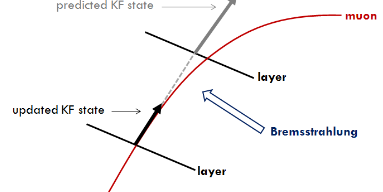
\includegraphics[width=0.60\textwidth]{figures/energyloss.png}
\caption{Representaci\'on gr\'afica del cambio en la trayectoria del mu\'on tras una gran p\'erdida de energ\'ia.}
\label{fig:energyloss}        
\end{figure}


\subsection{Asignaci\'on final de momento: el Algoritmo TuneP}\label{sec:TuneP}

Finalmente, la recomendaci\'on central de la colaboraci\'on CMS para el momento transverso de los muones high-$p_{T}$ se corresponde con el proporcionado por el algoritmo TuneP. El objetivo de este algoritmo es simplemente eligir cu\'al es la mejor reconstrucci\'on de la traza posible de entre la traza reconstruida \'unicamente en el tracker, y las trazas obtenidas por los distintos refits (TPFMS, Picky y DYT). La elecci\'on se hace conjuntamente en base al $\chi$\textsuperscript{2}/ndof y el $\sigma_{p_{T}}/p_{T}$ de las distintas trazas.
